
%%% Local Variables:
%%% mode: latex
%%% TeX-master: "gis18"
%%% End:



\section{Preliminaries}
\label{sec-pre}

In this section, we first introduce some basic concepts for trajectory tracking.
Then we introduce position and trajectory tracking algorithms \ldr and \ldrh that are helpful to understand the basic ideas of the work.
Notations used are summarized in Table \ref{tab:notations}.

\begin{table}
	\renewcommand{\arraystretch}{1.20}
	\caption{\small Summary of notations}
	\vspace{-1ex}
	\centering
	\footnotesize
	%\scriptsize
	\begin{tabular}{|c|l|}
		\hline
		{\bf Notations}& {\bf Semantics}   \\		\hline %\hline
		$P$ & a data point \\		\hline
		$\dddot{\mathcal{T}}$ & a trajectory $\dddot{\mathcal{T}}$ is a sequence of data points\\		\hline
		$\overline{\mathcal{T}}$&  {a piece-wise line representation of a trajectory $\dddot{\mathcal{T}}$}	\\		\hline
		$\mathcal{L}$ & a line segment  \\		\hline
		$\epsilon$ & an error bound \\		\hline
		$ped\left(P, \mathcal{L}\right)$ &  {the perpendicular Euclidean distance of point $P$ to line segment $\mathcal{L}$}	\\	\hline
		$sed\left(P, \mathcal{L}\right)$ & {the synchronous Euclidean distance of point $P$ to line segment $\mathcal{L}$} 	\\		\hline
		%$dad\left(\mathcal{L}_1, \mathcal{L}_2\right)$ & {the direction-aware distance of line segment $\mathcal{L}_1$ to line segment $\mathcal{L}_2$} 	%\\		\hline
		\sector{} & a sector \\		\hline
		%		$\overline{A} \times \overline{B}$ & the cross product of (vectors) $\overline{A}$ and $\overline{B}$\\		\hline
		%		$\mathcal{H}(\mathcal{L})$ & The open half-plane to the left of $\mathcal{L}$ \\		\hline
		%		$\mathcal{R}$& a convex polygon \\		\hline
		%		$\mathcal{R}^*$ & the intersection of convex polygons \\		\hline
		%		$m$ & the maximum number of edges of a polygon\\		\hline
		%		$E^j$ & a group of edges labeled with $j$\\		\hline
		%		$g(e)$ & the label of an edge $e$ of polygons \\		\hline
		%		\circle{} & a synchronous circle\\		\hline
		\cone{} & a spatio-temporal cone \\		\hline
		\circle{} & a synchronous circle \\		\hline
		%\pcircle{} & a cone projection circle \\		\hline
		$\mathcal{R}$& a convex polygon \\		\hline
		%$\mathcal{R}^*$ & the intersection of convex polygons \\		\hline
		%$\bigsqcap$ & intersection of geometries\\		\hline
		%$G$ &	the reachability graph of a trajectory\\		\hline
	\end{tabular}
	\label{tab:notations}
	\vspace{-1ex}
\end{table}


\begin{figure}[tb!]
	\centering
	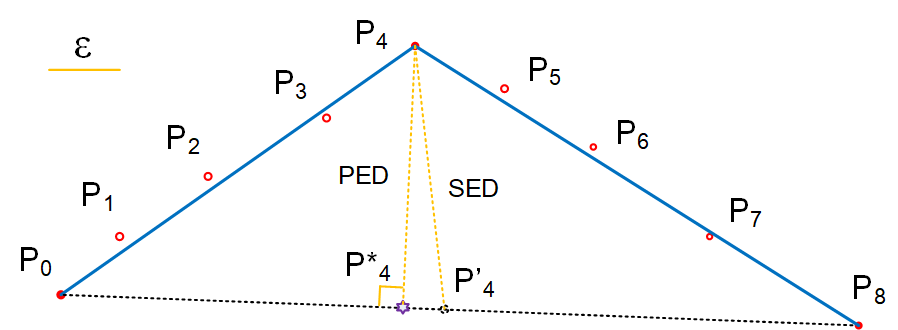
\includegraphics[scale=0.9]{Figures/Fig-Concepts.png}\vspace{-1ex}
	\caption{\small  A trajectory $\dddot{\mathcal{T}}[P_0, \ldots, P_{8}]$ with 9 points is simplified to (or represented by) two continuous line segments $ \overline{\mathcal{T}}[\overline{P_0P_4}, \overline{P_4P_{8}}] $ using \ped and \sed, respectively. In which, (1) $ped(P_4, \overline{P_0P_{8}})=|\overline{P_4P^*_4}|$, where $P^*_4$ is the perpendicular point of $P_4$ \wrt line segment $\overline{P_0P_{8}}$, and (2) $sed(P_4, \overline{P_0P_{8}})= |\overline{P_4P'_4}|$, where $P'_4$ is the synchronized point of $P_4$ \wrt $\overline{P_0P_{8}}$ satisfies ${|\overline{P_0P'_4}|}/{|\overline{P_0P_{8}}|} = \frac{(P_4.t - P_0.t)}{(P_{8}.t-P_0.t)} = \frac{(4-0)}{(8-0)}= \frac{1}{2}$.}
	\vspace{-1ex}
	\label{fig:concepts}
\end{figure}


\subsection{Notations}

We first introduce basic notations. They are illustrated with examples shown in {Figure}~\ref{fig:concepts}.

\stitle{Trajectory}. A \textit{trajectory} $\dddot{\mathcal{T}}\left[P_0, \ldots, P_n\right]$ is a sequence of points in a monotonically increasing order of their associated time values (\ie $P_i.t < P_j.t$ for any $0\le i<j\le n$), where a data \textit{point} is defined as a triple $P\left(x, y, t\right)$, which represents that a moving object is located at {\em longitude} $x$ and {\em latitude} $y$ at {\em time} $t$. 
%Note that data points can be viewed as points in a three-dimension Euclidean space.


\eat{%%%%%%%%%%%%%%%%%%%%
	A \textit{line segment} (or line segment for simplicity) $\mathcal{L}$ is defined as $\overline{P_{s}P_{e}}$, which represents the closed line segment that connects the start point $P_s$ and the end point $P_e$.
	We also use $|\mathcal{L}|$ and $\mathcal{L}.\theta\in [0, 2\pi)$ to denote the length of a line segment $\mathcal{L}$, and its angle with the $x$-axis of the coordinate system $(x, y)$, where $x$ and $y$ are the longitude and latitude, respectively.
	That is, a line segment $\mathcal{L}$ = $\overline{P_{s}P_{e}}$ can be treated as a triple $(P_s, |\mathcal{L}|, \mathcal{L}.\theta)$.
}%%%%%%%%%%%%%%%%%%%%%%

%Intuitively, a trajectory can also be represented by a continuous $n$-pieces line segments (or line segment for simplicity) $\mathcal{L}_i$, $0\le i < n$, where  $\mathcal{L}_i = \overline{P_{i}P_{i+1}}$, represents the closed line segment that connects the start point $P_{i}$ and the end point $P_{i+1}$.

\stitle{Piece-wise line representation}. A \textit{piece-wise line representation} $\overline{\mathcal{T}}\left[\mathcal{L}_0, \ldots, \mathcal{L}_m\right]$ ($0< m \le n$) of a trajectory $\dddot{\mathcal{T}}\left[P_0, \ldots, P_n\right]$ is a sequence of continuous \textit{line segments} $\mathcal{L}_{i}$ = $\overline{P_{s_i}P_{e_i}}$ ($i\in\left[0,m\right]$) of $\dddot{\mathcal{T}}$ such that $\mathcal{L}_{0}.P_{s_0} = P_0$, $\mathcal{L}_{m}.P_{e_m} = P_n$ and  $\mathcal{L}_{i}.P_{e_i}$ = $\mathcal{L}_{i+1}.P_{s_{i+1}}$ for all $i\in\left[0, m-1\right]$.
Note that each line segment in $\overline{\mathcal{T}}$ essentially represents a continuous sequence of data points in trajectory $\dddot{\mathcal{T}}$.


For trajectory simplification, two Euclidean distance metrics are commonly used, namely, the \emph{perpendicular Euclidean distance} (\ped) and the \emph{synchronous Euclidean distance} \cite{Meratnia:Spatiotemporal} (\sed). Among them, \sed is also used in position and trajectory tracking.
%
Consider a data point $P$ and a line segment $\mathcal{L}$ = $\overline{P_{s}P_{e}}$.

\stitle{Perpendicular Euclidean distance}. The perpendicular Euclidean distance $ped\left(P, \mathcal{L}\right)$ of point $P$ to line segment $\mathcal{L}$ is $\min\{|PQ|\}$ for any point $Q$ on $\overline{P_{s}P_{e}}$.

\stitle{Synchronous Euclidean distance}. The synchronous Euclidean distance $sed\left(P, \mathcal{L}\right)$ of point $P$ to line segment $\mathcal{L}$ is $|\overline{PP'}|$ that is the Euclidean distance from $P$ to its \textit{synchronized point} $P'$ \wrt $\mathcal{L}$, where the synchronized point $P'$ \wrt $\mathcal{L}$ is defined as follows:
(a) $P'.x$ = $P_s.x +  c\cdot\left(P_e.x - P_s.x\right)$,
(b) $P'.y$ = $P_s.y +  c\cdot\left(P_e.y - P_s.y\right)$ and
(c) $P'.t$ = $P.t$, where $c= \frac{P.t-P_s.t}{P_e.t-P_s.t}$.

The \emph{synchronized point} $P'$ of a point $P$ \wrt line segment $\overline{P_sP_e}$ is the expected position of the moving object on $\overline{P_sP_e}$ at time $P.t$, obtained by a linear interpolation \cite{Cao:Spatio} that assumes it moved along the straight line from $P_s$ to $P_e$ with a uniform speed of $\frac{|\overline{P_sP_e}|}{P_e.t-P_s.t}$.


%Synchronized points are essentially virtual points with the assumption that an object moved along a straight line from $P_s$ to $P_e$ with a uniform speed, \ie the average speed $\frac{|\overline{P_sP_e}|}{P_e.t-P_s.t}$ between points $P_s$ and $P_e$ \cite{Cao:Spatio,Lin:Cised}. 

%More specifically, a synchronized point $P'_i$ of $P_i$ ($s\le i < e$) \wrt the line segment $\overline{P_sP_e}$ is a point on $\overline{P_sP_{e}}$ satisfying ${|\overline{P_sP'_i}|} = \frac{P_i.t - P_s.t}{P_e.t - P_s.t}\cdot {|\overline{P_sP_e}|}$, which means that the object moves from $P_s$ to $P_e$ at an average speed $\frac{|\overline{P_sP_e}|}{P_e.t-P_s.t}$, and its position at time $P_i.t$ is the point $P'_i$ on $\overrightarrow{P_sP_{e}}$ having a distance of $\frac{P_i.t - P_s.t}{P_e.t - P_s.t}\cdot|\overline{P_sP_e}|$ to $P_s$~\cite{Cao:Spatio, Lin:Cised,Meratnia:Spatiotemporal, Chen:Fast, Zhang:Evaluation}.






 
 


\eat{%%%%%%%%%%%%%%
\begin{example}
	\label{exm-notations}
	Consider {Figure}~\ref{fig:concepts}, in which
	%
	(1) $\dddot{\mathcal{T}}\left[P_0, \ldots, P_{8}\right]$ is a trajectory having 9 data points,
	%
	(2) a set of two continuous line segments $\{\overline{P_0P_4}$, $\overline{P_4P_{8}}$\} is a piece-wise line representation of trajectory $\dddot{\mathcal{T}}$,
	%
	(3) $ped\left(P_4, \overline{P_0P_{8}}\right)=|\overline{P_4P^*_4}|$, where $P^*_4$ is the perpendicular point of $P_4$ \wrt line segment $\overline{P_0P_{8}}$, and 
	%
	(4) $sed\left(P_4, \overline{P_0P_{8}}\right)= |\overline{P_4P'_4}|$,
	where $P'_4$ is the synchronized point of $P_4$ \wrt $\overline{P_0P_{8}}$ satisfies $\frac{|\overline{P_0P'_4}|}{|\overline{P_0P_{8}}|} = \frac{P_4.t - P_0.t}{P_{8}.t-P_0.t} = \frac{4-0}{8-0}= \frac{1}{2}$.
\end{example}
}%%%%%%%%%%%%eat

\eat{%%%%%%%%%%%%%%%%%%
\stitle{Direction-aware distance distance}.The direction-aware distance $dad\left(\mathcal{L}_1, \mathcal{L}_2\right)$ is the direction deviation from $\mathcal{L}_1$ to $\mathcal{L}_2$, \ie $\Delta\left(\mathcal{L}_1.\theta, \mathcal{L}_2.\theta\right) = \min\{|\mathcal{L}_1.\theta - \mathcal{L}_2.\theta|, 2\pi - |\mathcal{L}_1.\theta - \mathcal{L}_2.\theta|\}$, where $\theta \in \left[0, 2\pi\right)$ is the angular of $\mathcal{L}$.
\textcolor{blue}{Note \dad differs from \ped and \sed in that it is a measure of angle, rather than Euclidean distances, and the temporal information is also lost when using \dad.}

\stitle{Trajectory simplification (Min-$\#$ problem).}
Given a trajectory \trajec{T}$\left[P_0, \dots, P_n\right]$ and a pre-specified constant $\epsilon$, the \emph{min-$\#$} problem of trajectory simplification is to approximate the trajectory \trajec{T} with $\overline{\mathcal{T}}\left[\mathcal{L}_0, \ldots , \mathcal{L}_m\right]$ ($0< m \le n$), such that
(1) on each of them the points $\left[P_{s_i}, \dots, P_{e_i}\right]$ are approximated by a line segment $\mathcal{L}_i = \overline{P_{s_i}P_{e_i}}$ with the maximum \ped or \sed \emph{error} of point $P_j$ (or \dad \emph{error} of line segment $|\overline{P_jP_{j+1}}|$) to line segment $\mathcal{L}_i$, $s_i \le j<e_i$,  less than $\epsilon$, and
(2) $P_{s_i}$ and $P_{e_i} \in$ \trajec{T}.


\stitle{Position tracking}. \textcolor{blue}{Given an error bound $\epsilon$, the position tracking is an agreement between a moving object and a MOD server such that the MOD server can infer the current position of the object with an deviation less than $\epsilon$ to its actual position.}

\stitle{Trajectory tracking}. It is a method implementing both trajectory simplification and position tracking.
}%%%%%%%%%%End EAT

\subsection{Position tracking in a floating disc}

\textit{Position tracking} aims at informing the MOD about the current position of an object. Currently, the most simple yet efficient position tracking protocols is linear dead reckoning (\ldr) \cite{Wolfson:PositionTracking}, which is essentially an agreement between a moving object and a MOD server such that given an initial position $P_s$, a velocity $\vv{v}$ and a user specified threshold $\epsilon$, the server could infer the current position $P'$ of the object based on $P_s$ and $\vv{v}$ such that the distance from $P'$ to the actual position $P$ of the object is bounded by the threshold $\epsilon$. A moving object only reports its position at the time $|P'P| \ge \epsilon$, \ie the object's locally sensed position impends to deviate from the expected one by more than the threshold \cite{Lange:Tracking}. By this way, the number of messages is reduced.
%essentially an agreement between a given moving object and the MOD server whose purpose is to let the MOD server track a moving object with less communication between them at an expense of imprecise of position within an error bound $\epsilon$.  


Given an error bound $\epsilon$, the moving object sends its initial location $P_s$ and the expected velocity $\vv{v}$
(including value and direction) to the MOD server, meaning that it is supposed to move from $P_s$ along the direction of $\vv{v}$ at a speed of $|\vv{v}|$, such that the expected position (\ie synchronized point) of the object at time $t>t_s$ can be extrapolated from them as long as no subsequent update is sent to the MOD server. 
After that, because the actual speed of it may be varied and different from the supposed speed of $|\vv{v}|$, the moving object periodically collects its actual position by sampling its on-board sensor, \eg GPS, and compares the actual position of time $t$ with the expected position of time $t$ extrapolated from the initial position $P_s$ and the velocity $\vv{v}$. 
If the deviation from its actual position to the expected position (\ie the synchronous Euclidean distance) is not more than $\epsilon$, then the object does not transmit any new updates to MOD, otherwise, an update of new ($P_s$, $\vv{v}$) will be sent.
%
By this way, though the MOD server receives less position information about a moving object, it still knows the expected position of the moving object with a bounded error of $\epsilon$ to its actual position. The \ldr mechanism ensures that no message is sent as long as the actual position $P$ is in a circular area around the excepted position $P'$ with a radius of $\epsilon$. That is, \emph{\ldr tracks a moving object inside a floating disc having a velocity of $\vv{v}$.}

\begin{figure}[tb!]
	\centering
	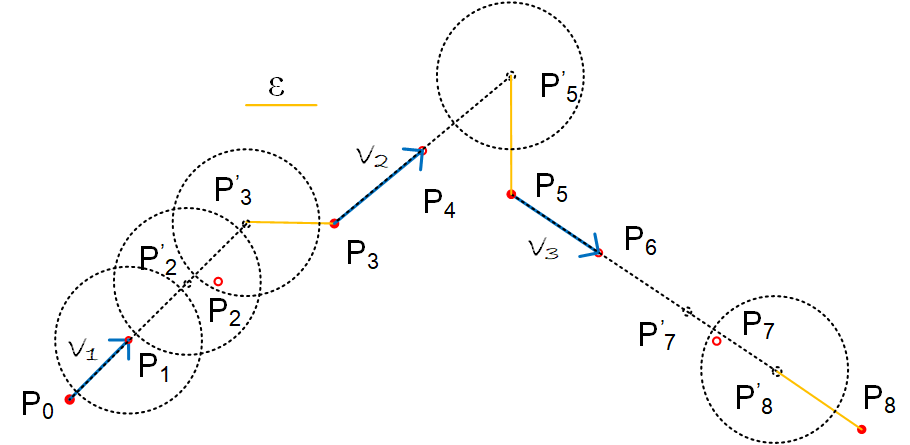
\includegraphics[scale=0.9]{figures/Fig-LDR.png}
	\vspace{-1ex}
	\caption{\small A running example of position tracking by \ldr. }
	\vspace{-2ex}
	\label{fig:ldr}
\end{figure}

\begin{example}
	\label{exm-ldr}
Figure \ref{fig:ldr} is a running example of \ldr.
Initially, point $P_0$ is set as $P_s$ and $\vec{v}$ is set to $\vec{v}_0$. Then, (1) points $P_1$ and $P_2$ have \sed distances less than $\epsilon$ to their expected points $P'_1$ and $P'_2$, respectively, and (2) $|P_3P'_3| > \epsilon$, meaning $P_3$ breaks the distance threshold, thus, a new update is triggered and $P_3$ is the new start point of the next section of position tracking.
%
\end{example}

%This example also demonstrates that (1) the expected position is indeed the synchronized point of the moving object at time $t$, (2) the deviation from the actual position to the expected position \wrt $\vv{v}$ is sure the synchronous Euclidean distance (\sed), and (3) 

 




\subsection{Trajectory tracking in a floating disc}
\textit{Trajectory tracking} aims to implement both position tracking and trajectory simplification in one routine \cite{Lange:Tracking}. Currently, the one-pass trajectory tracking algorithm is a variation of \ldr, originally developed in \cite{Trajcevski:LDRH} and formally named as linear dead reckoning with half $\epsilon$ (\ldrh) in \cite{Lange:Tracking}.
%
Authors in \cite{Trajcevski:LDRH} proved that \ldr with some small variations is also a line simplification algorithm. Thus, \ldrh supports both position tracking and trajectory simplification, meaning it is a trajectory tracking algorithm.

Given an error bound $\epsilon$, \ldrh runs the same routine as \ldr except that (1) it uses half $\epsilon$ as the threshold in distance checking; (2) when the current point $P_k$ has a \sed larger than $\epsilon/2$ to its expected location (synchronous data point), it sends the preview point $P_{k-1}$ and a new $\vv{v}$ to the MOD server and continues trajectory tracking taking $P_{k-1}$ as the new start point. \ldrh is simple and efficient, having a linear time and a constant space. However, it has a poor effectiveness in terms of compression ratio, as the half $\epsilon$ is conservative, and more important, the algorithm is sensitive to the initial velocity which is set at the updating time but it is hard to be appropriate when the process goes on.

\begin{example}
Figure~\ref{fig:ldrh} is a running example of \ldrh taking the same input as Figure \ref{fig:ldr}.
Initially, the start point $P_s$ is set to $P_0$ and the velocity $\vec{v}$ is set to $\vec{v}_0$. Then, (1) $P_1$ and $P_2$ have \sed distances less than $\epsilon/2$ to their expected points $P'_1$ and $P'_2$, respectively, (2) $|P_3P'_3| > \epsilon/2$, thus, a new update is triggered and $P_2$ is the new start point of the next section of trajectory tracking. Finally, this algorithm in turn sends 5 points, $P_0, P_2, P_4, P_6$ and $P_8$, and 4 velocities, $\vec{v_1}$, $\vec{v_2}$, $\vec{v_3}$ and $\vec{v_4}$, to the MOD server.
\end{example}

\begin{figure}[tb!]
	\centering
	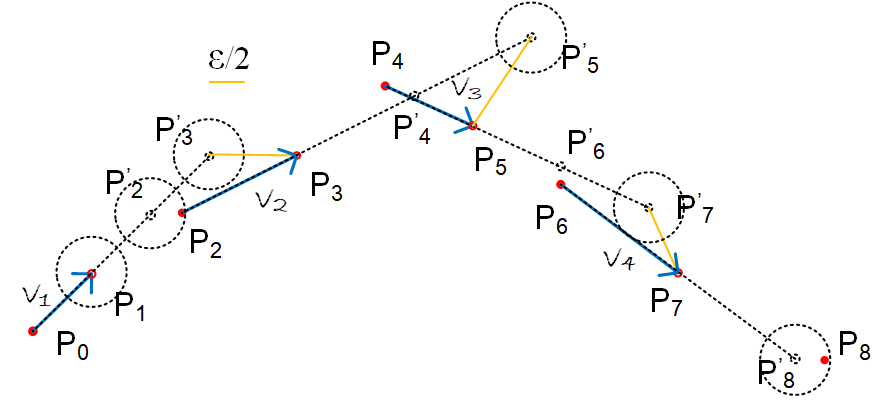
\includegraphics[scale=1.0]{figures/Fig-LDRH.png}
	\vspace{-1.5ex}
	\caption{\small A running example of trajectory tracking by \ldrh. }
	\vspace{-2ex}
	\label{fig:ldrh}
\end{figure}

%%%%%%
\eat{ 
	\textcolor{blue}{ 
		Lange et al. in \cite{Lange:GRTS, Lange:Tracking} introduced \grts framework that aimed at improving the effectiveness, in terms of compression ratio, of trajectory tracking by logically separating position tracking and trajectory simplification into two sub-processes, where position tracking is implemented by \ldr and trajectory simplification is enforced by integrating the third party line simplification algorithms \cite{Zhang:Evaluation, Lin:Cised}. \grts is effective than \ldrh, however, it is much more complex as it includes two sub-processes and introduces a buffer to temporarily save data points for the purpose of compression.
		Like \ldr, algorithms \ldrh and \grts both use \sed to check distances, hence, they also track a moving object in a floating circular area.}
}
%%%%%%eat









%\subsection{Trajectory simplification in strip areas}
%\todo{sleeve (half-epsilon)}

